% !TEX options=--shell-escape
\pdfobjcompresslevel=0
\documentclass[slidetop,11pt]{beamer}
\usepackage[utf8]{inputenc}
\usepackage{dsfont}
\usepackage{multirow}
\usepackage{array}
\usepackage{xcolor}
\usepackage{algorithmic}
\usepackage[plain]{algorithm}
\usepackage{ulem}
\usepackage{mathabx}
\usepackage{graphicx}
% declare the path(s) where your graphic files are
\graphicspath{{img/}}
\DeclareGraphicsExtensions{.pdf,.jpeg,.png,.eps}
\usepackage{subfig}
\usepackage{soul} % strikethrough
\usepackage{minted}


\usetheme{progressbar}
\setbeamertemplate{footline}[frame number]
\setbeamercovered{transparent}
\useinnertheme{default}

\newcommand{\mv}{{\rm  MV}}

\DeclareMathOperator*{\argmin}{\arg\!\min}
\DeclareMathOperator*{\sgn}{\text{sgn}}

\newtheorem{prop}{Property}
\newtheorem{thm}{Theorem}
\newtheorem{rem}{Remark}

\newenvironment{changemargin}[2]{%
  \begin{list}{}{% 
    \setlength{\topsep}{0pt}% 
    \setlength{\leftmargin}{#1}% 
    \setlength{\rightmargin}{#2}% 
    \setlength{\listparindent}{\parindent}% 
    \setlength{\itemindent}{\parindent}% 
    \setlength{\parsep}{\parskip}% 
  }% 
  \item[]}{\end{list}}

\makeatletter
\newcommand{\vast}{\bBigg@{3}}
\makeatother
	
\definecolor{dgreen}{rgb}{0.,0.6,0.}
\definecolor{azure}{rgb}{0.,0.5,1.}
\definecolor{bluegray}{rgb}{0.4,0.6,0.8}
\definecolor{bleu}{rgb}{0.19,0.55,0.91}

\newcommand{\semitransp}[2][30]{\color{fg!#1}#2}


\title{{\large Anomaly detection in scikit-learn} \\ {\normalfont \small{Ongoing work and future developments}}}
\author{Albert Thomas}
\institute{T\'el\'ecom ParisTech - Huawei Technologies}


\begin{document}

\captionsetup[subfigure]{labelformat=empty}

\begin{frame}

\includegraphics[width=2.3cm]{img/scikit-learn-logo-notext.png}
% \hspace{6.7cm}
% \includegraphics[width=1cm]{img/logo_telecom.jpg}
\titlepage

\end{frame}


\begin{frame}
\frametitle{Anomaly detection}

\begin{itemize}
\item \textbf{Imbalanced classification}: anomalies and normal data available, usually highly imbalanced data set

\item \textbf{Novely detection}: normal data available, fit on normal data, then predict on unlabelled data

\item \textbf{Outlier detection}: unlabelled data only, fit \textbf{and} predict on unlabelled data. Anomalies are rare events, located in the low density regions.
\end{itemize}

\begin{center}
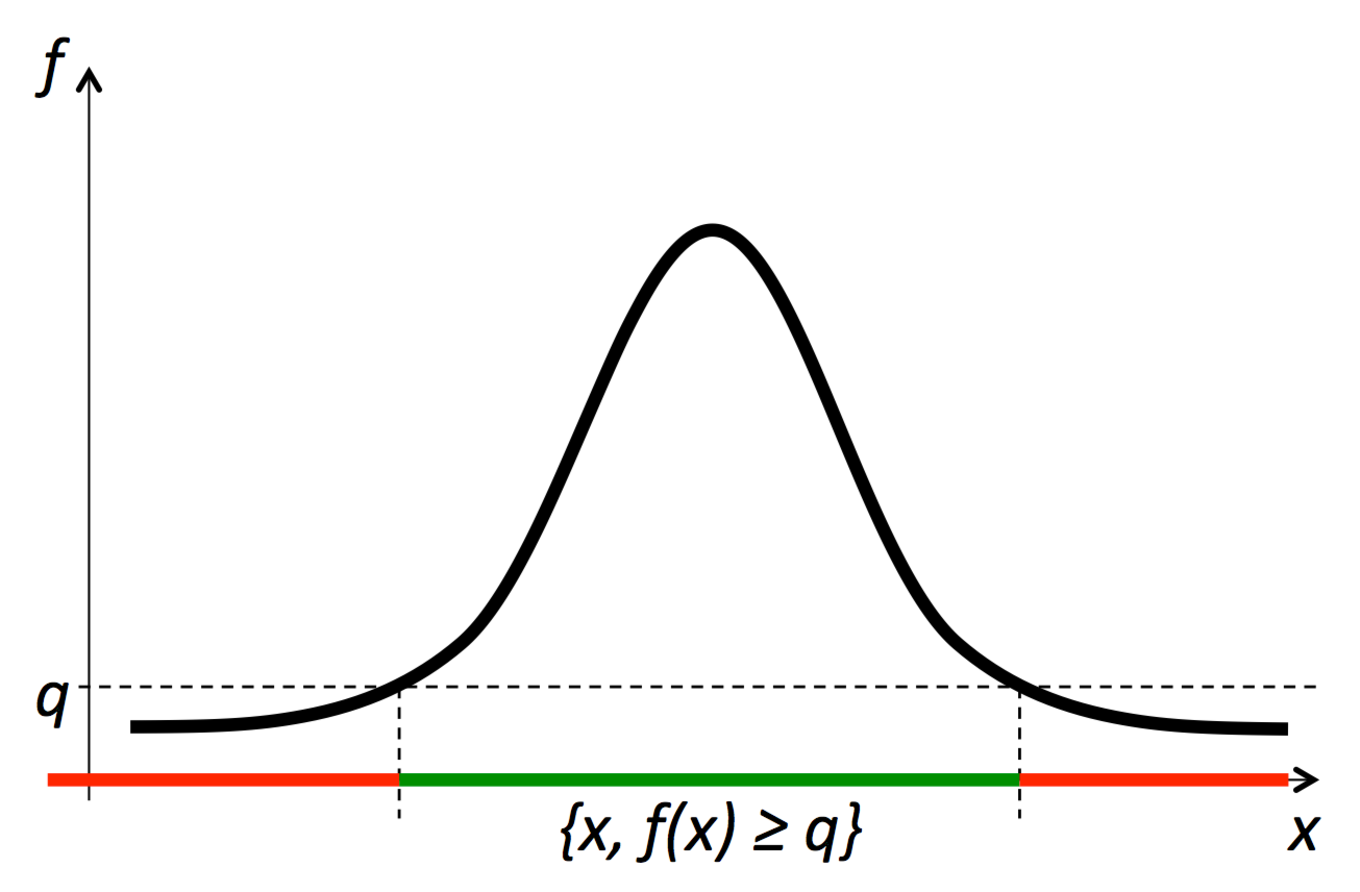
\includegraphics[width=5cm]{dls3.pdf}
\end{center}

\begin{center}
Find the \textbf{high density regions}
\end{center}

\end{frame}



\begin{frame}
\frametitle{Outlier and novelty detection algorithms}

Common approach

\vspace{0.5cm}

\begin{enumerate}
\item[1.] Learn a scoring function $s$ such that
\begin{center}
the smaller $s(x)$ the more abnormal is $x$
\end{center}

\vspace{0.5cm}

\item[2.] Threshold $s$ at an offset $q$ such that outlier/novelties are such that
\begin{equation*}
\{x, s(x) < q \}
\end{equation*}
$q$ usually depends on a \mintinline{python}{contamination} parameter
\end{enumerate}

\begin{center}
EllipticEnvelope, OneClassSVM \\
IsolationForest (iForest) and LocalOutlierFactor (LOF)
\end{center}

\end{frame}


\begin{frame}\frametitle{Algorithms}
    
\begin{center}
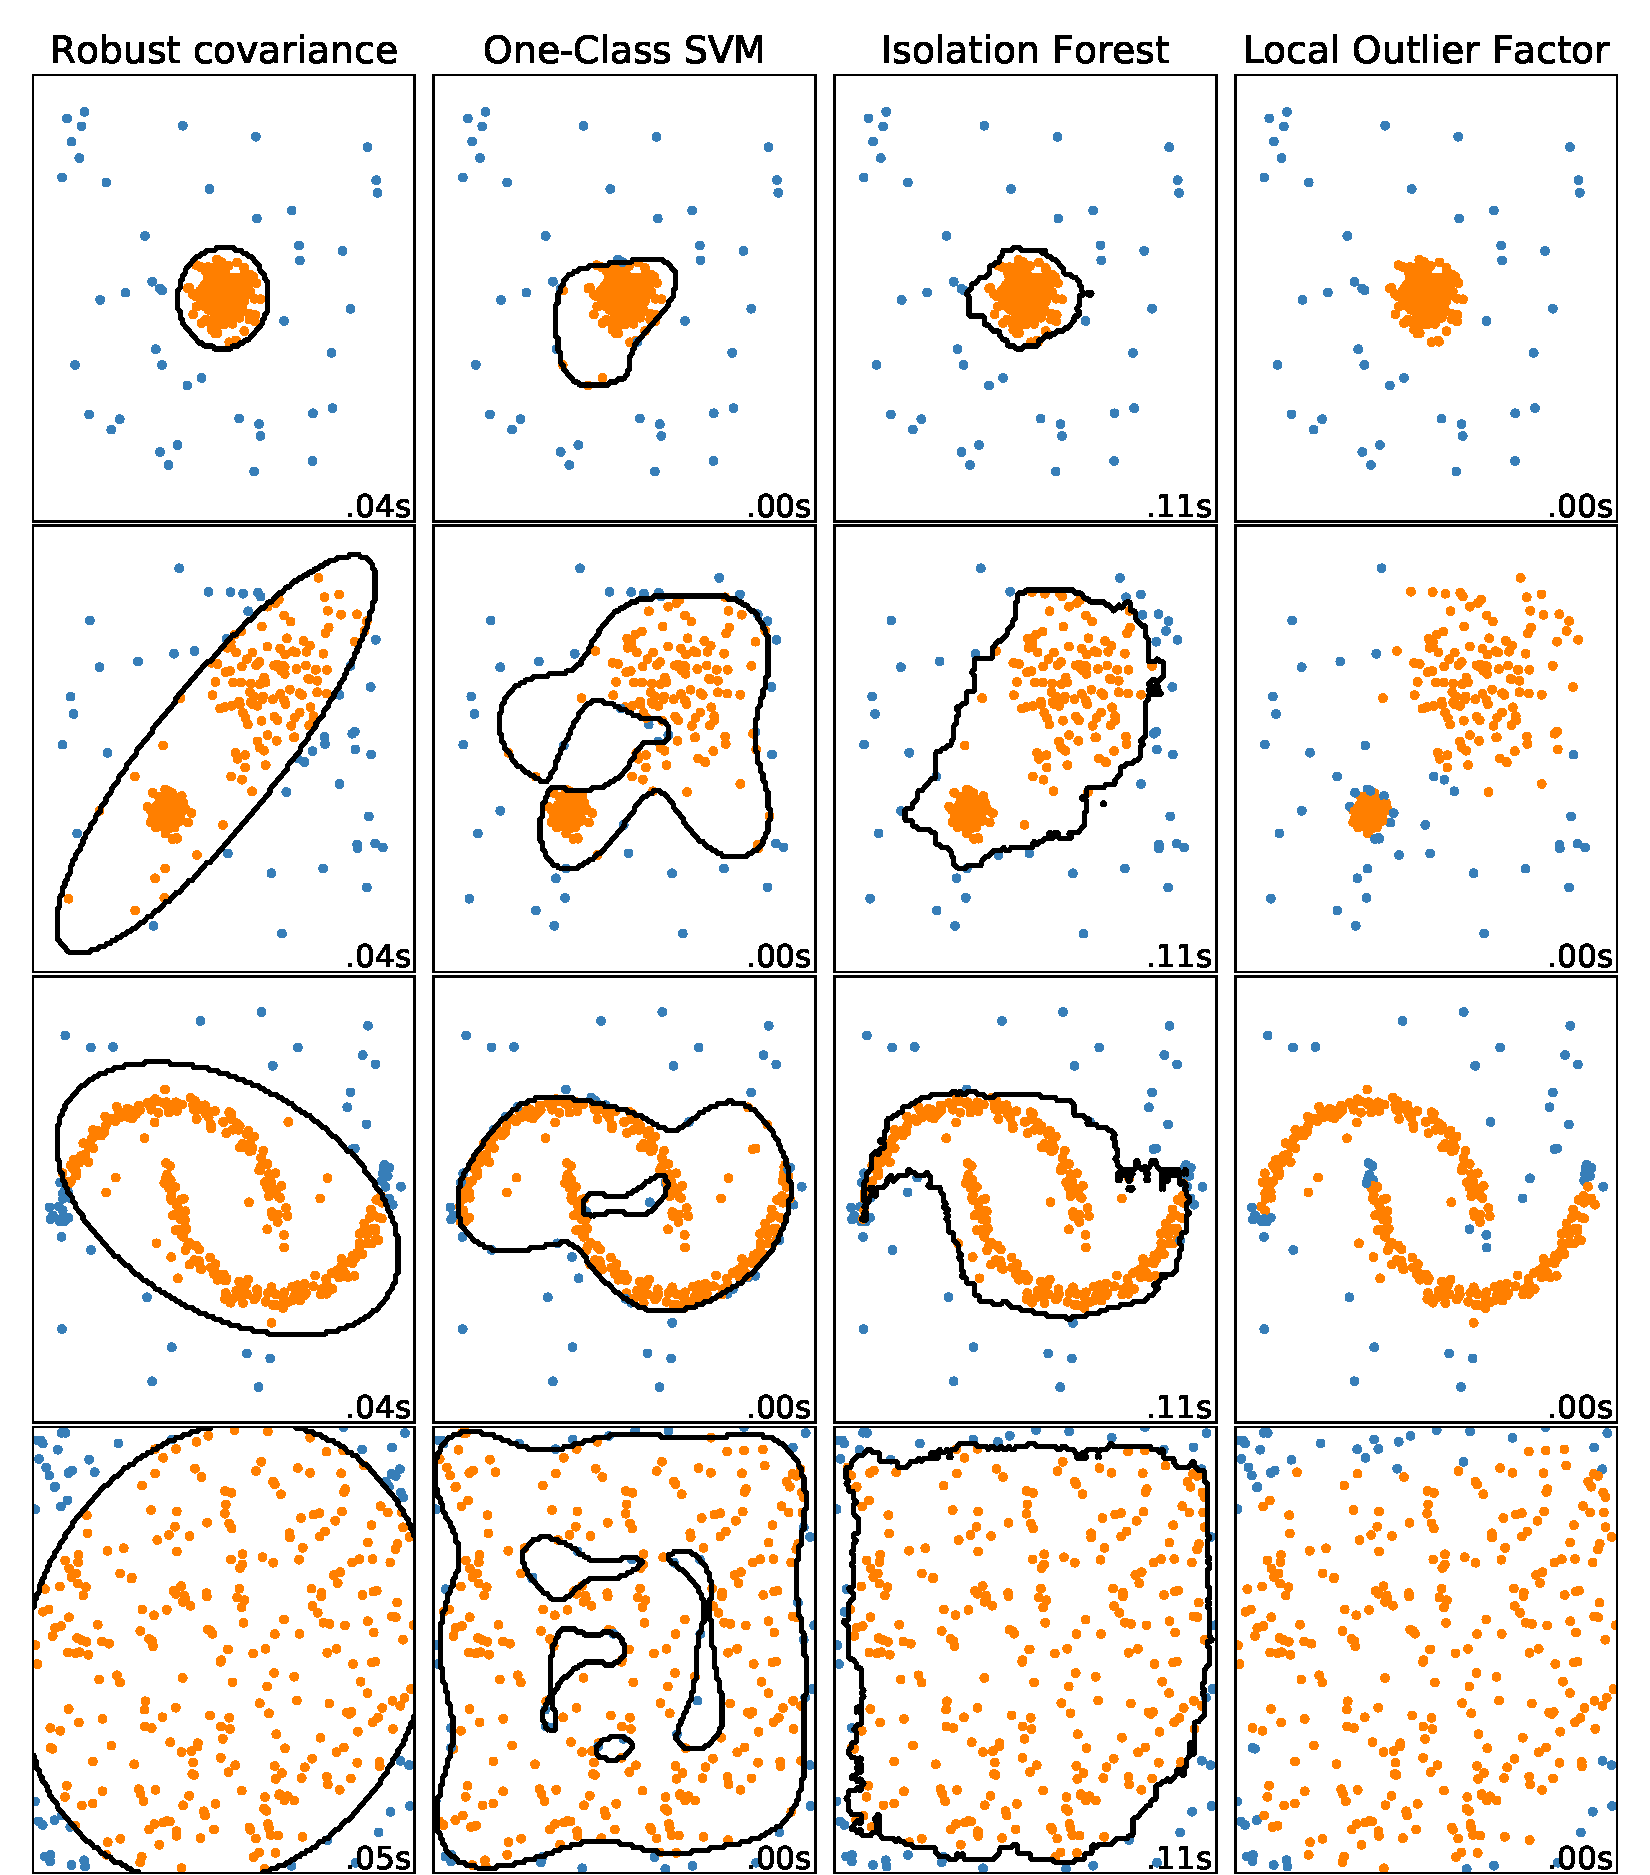
\includegraphics[width=6.8cm]{img/anomaly_comparison.pdf}
\end{center}

\end{frame}


\begin{frame}\frametitle{Scikit-learn API}
    
\begin{center}
PR on \textbf{API consistency} $\vcenter{\hbox{
\includegraphics[width=1.7cm]{img/merged_logo.pdf}}}$ last week
\end{center}

\begin{itemize}
  \item \mintinline{python}{decision_function}
  \item new \mintinline{python}{score_samples} method
\end{itemize}

\end{frame}


\begin{frame}\frametitle{Scikit-learn API}

EllipticEnvelope, OneClassSVM and IsolationForest

\onslide<1->{
\begin{itemize}
  \item instantiate your estimator, e.g.~\mintinline{python}{clf = OneClassSVM()}
  \item \mintinline{python}{clf.fit(X_train)}
  \item \mintinline{python}{clf.score_samples(X_test)}: raw score $s$
  \item \mintinline{python}{clf.decision_function(X_test)}: thresholded score
  \begin{equation*}
  \mintinline{python}{clf.score_samples(X_test) - clf.offset_} \quad
  \begin{cases}
    \geq 0 \quad \text{for inliers} \\
    < 0 \quad \text{for outliers}
  \end{cases}
  \end{equation*}
  \item \mintinline{python}{clf.predict(X_test)}
  \begin{equation*}
  \begin{cases}
    +1 \quad \text{for inliers} \\
    -1 \quad \text{for outliers}
  \end{cases}
  \end{equation*}
\end{itemize}
}

\visible<2>{
\begin{center}
\alert{Not valid for LOF}
\end{center}
}

\end{frame}


\begin{frame}\frametitle{Scikit-learn API - Outlier detection}

LOF, based on \mintinline{python}{k}-NN distances

\begin{itemize}
  \item \mintinline{python}{predict} on \mintinline{python}{x} $\in$ \mintinline{python}{X_train}: take \mintinline{python}{k} nearest neighbors of \mintinline{python}{x} in $\mintinline{python}{X_train} \setminus \mintinline{python}{x}$
  \item \mintinline{python}{predict} on \mintinline{python}{x} $\notin$ \mintinline{python}{X_train}: take \mintinline{python}{k} nearest neighbors of \mintinline{python}{x} in \mintinline{python}{X_train}
\end{itemize}
\begin{center}
Hard to check that $\mintinline{python}{x} \in \mintinline{python}{X_train}$ or not...
\end{center}

\end{frame}


\begin{frame}\frametitle{Scikit-learn API - Outlier detection}

\onslide<1->{
1st solution
\begin{itemize}
  \item \mintinline{python}{fit_predict(X_train)} to predict on \mintinline{python}{X_train}
  \item \mintinline{python}{predict(X_test)} to predict on \mintinline{python}{X_test}
\end{itemize}
}

\visible<2>{
\begin{center}
\alert{\mintinline{python}{fit(X).predict(X) != fit_predict(X)}}
\end{center}
}



\end{frame}



\begin{frame}\frametitle{Scikit-learn API - Outlier detection}

\onslide<1->{
2nd solution
\begin{itemize}
  \item only \mintinline{python}{fit_predict(X)} is public
  \item \mintinline{python}{_score_samples}, \mintinline{python}{_decision_function} and \mintinline{python}{_predict} are private
\end{itemize}
% LOF's original paper is only about outlier detection
}

\visible<2->{
\begin{center}
\textbf{Cannot (officialy) use LOF for novelty detection}
\end{center}
\vspace{0.4cm}
\begin{center}

\includegraphics[width=1.8cm]{img/shocking.jpg}
\end{center}
}

\end{frame}


\begin{frame}\frametitle{Scikit-learn API}

\onslide<1->{
\mintinline{python}{contamination} parameter in $(0, 1)$ (\mintinline{python}{nu} for OneClassSVM)

\begin{itemize}
  \item for outlier detection: proportion of outliers in the data set
  \item for novelty detection: type-I error (false positive rate)
\end{itemize}
}

\visible<2->{
Used to compute the offset $q$ on the training set
\begin{equation*}
\{s(x) < q \} = \{\text{\mintinline{python}{clf.score_samples(x) < clf.offset_}}\}
\end{equation*}
}
\visible<3->{
\mintinline{python}{contamination} can be set to \mintinline{python}{'auto'} for iForest and LOF
\begin{itemize}
  \item iForest: score of inliers close to 0 and score of outliers close to -1
  \begin{equation*}
  \mintinline{python}{clf.offset_ = -0.5}
  \end{equation*}
  
  \item LOF: score of inliers $\approx -1$
  \begin{equation*}
  \mintinline{python}{clf.offset_ = -1.5}
  \end{equation*}
\end{itemize}
}

\end{frame}


\begin{frame}\frametitle{Common tests}

$\vcenter{\hbox{
\includegraphics[width=1.4cm]{img/open_logo.pdf}}}$ PR on \textbf{common tests for outlier detection estimators}

\begin{itemize}
  \item Create an \mintinline{python}{OutlierDetectionMixin} for all outlier and novelty detection estimators: defines a \mintinline{python}{fit_predict}
  \item For all estimators test \mintinline{python}{fit_predict}: type, shape, \mintinline{python}{contamination}, \mintinline{python}{fit.predict = fit_predict}, labels $\in [-1, 1]$
  \item For novelty detection estimators: type, shape, \mintinline{python}{contamination}, \mintinline{python}{score_samples}, \mintinline{python}{decision_function}, \mintinline{python}{offset_}
\end{itemize}
  

\end{frame}


\begin{frame}[fragile]\frametitle{SGD OneClassSVM}

$\vcenter{\hbox{
\includegraphics[width=1.4cm]{img/open_logo.pdf}}}$ PR on \textbf{OneClassSVM using SGD}

\begin{itemize}
  \item Solves a linear version of the OneClassSVM: to pipeline with a kernel approximation
\end{itemize}

\begin{minted}{python}

  from sklearn.kernel_approximation import Nystroem
  from sklearn.linear_model import SGDOneClassSVM

  nystroem = Nystroem(gamma=gamma)
  online_ocsvm = SGDOneClassSVM(nu=nu)
  pipe_online = make_pipeline(nystroem, online_ocsvm)

  pipe_online.fit(X_train)

\end{minted}

\end{frame}


\begin{frame}\frametitle{SGD OneClassSVM}

$\vcenter{\hbox{
\includegraphics[width=1.4cm]{img/open_logo.pdf}}}$ PR on \textbf{OneClassSVM using SGD}

\only<1>{
\begin{center}
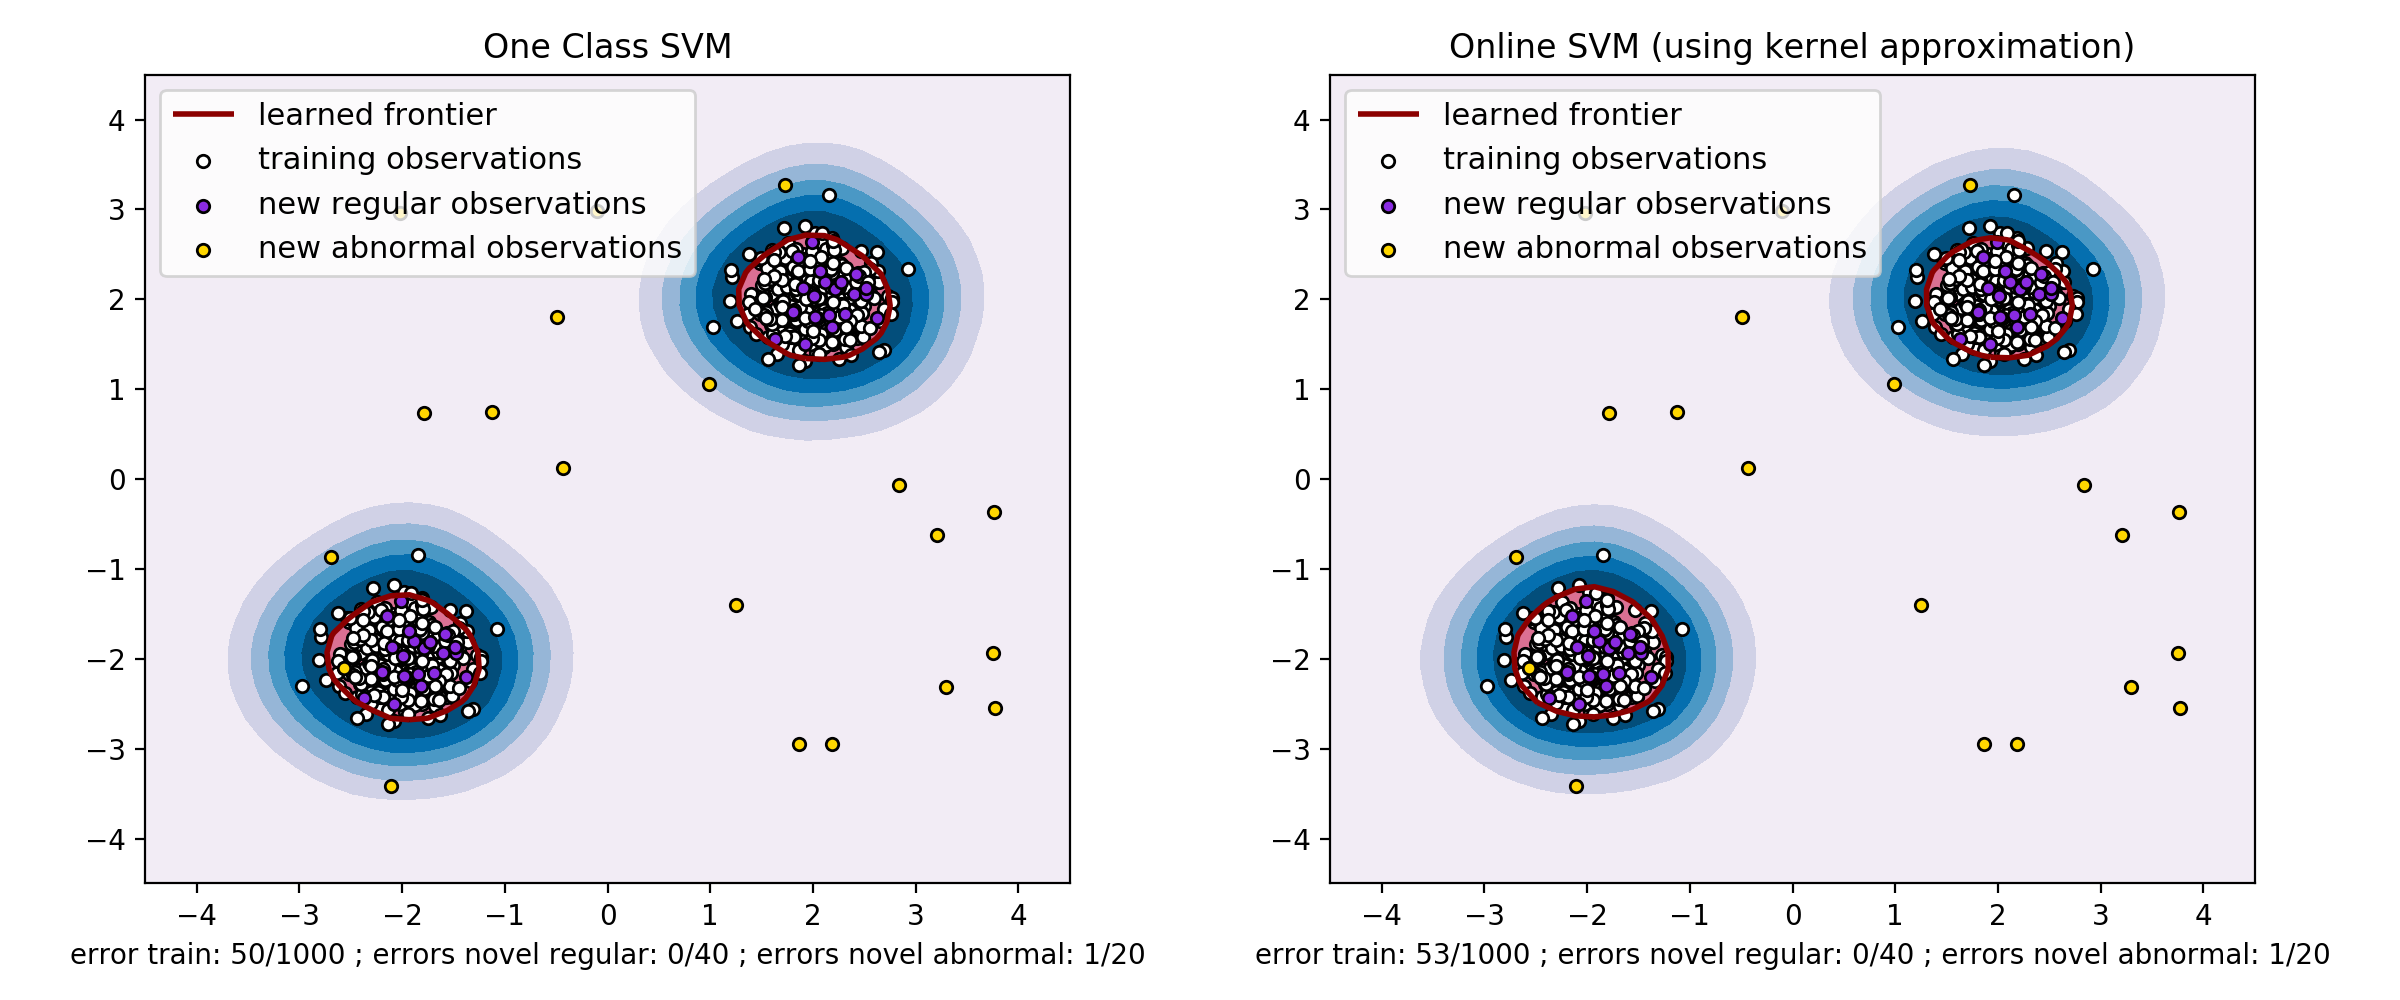
\includegraphics[width=11.5cm]{img/example_sgdocsvm.png}
\end{center}
}

\only<2>{
\begin{center}
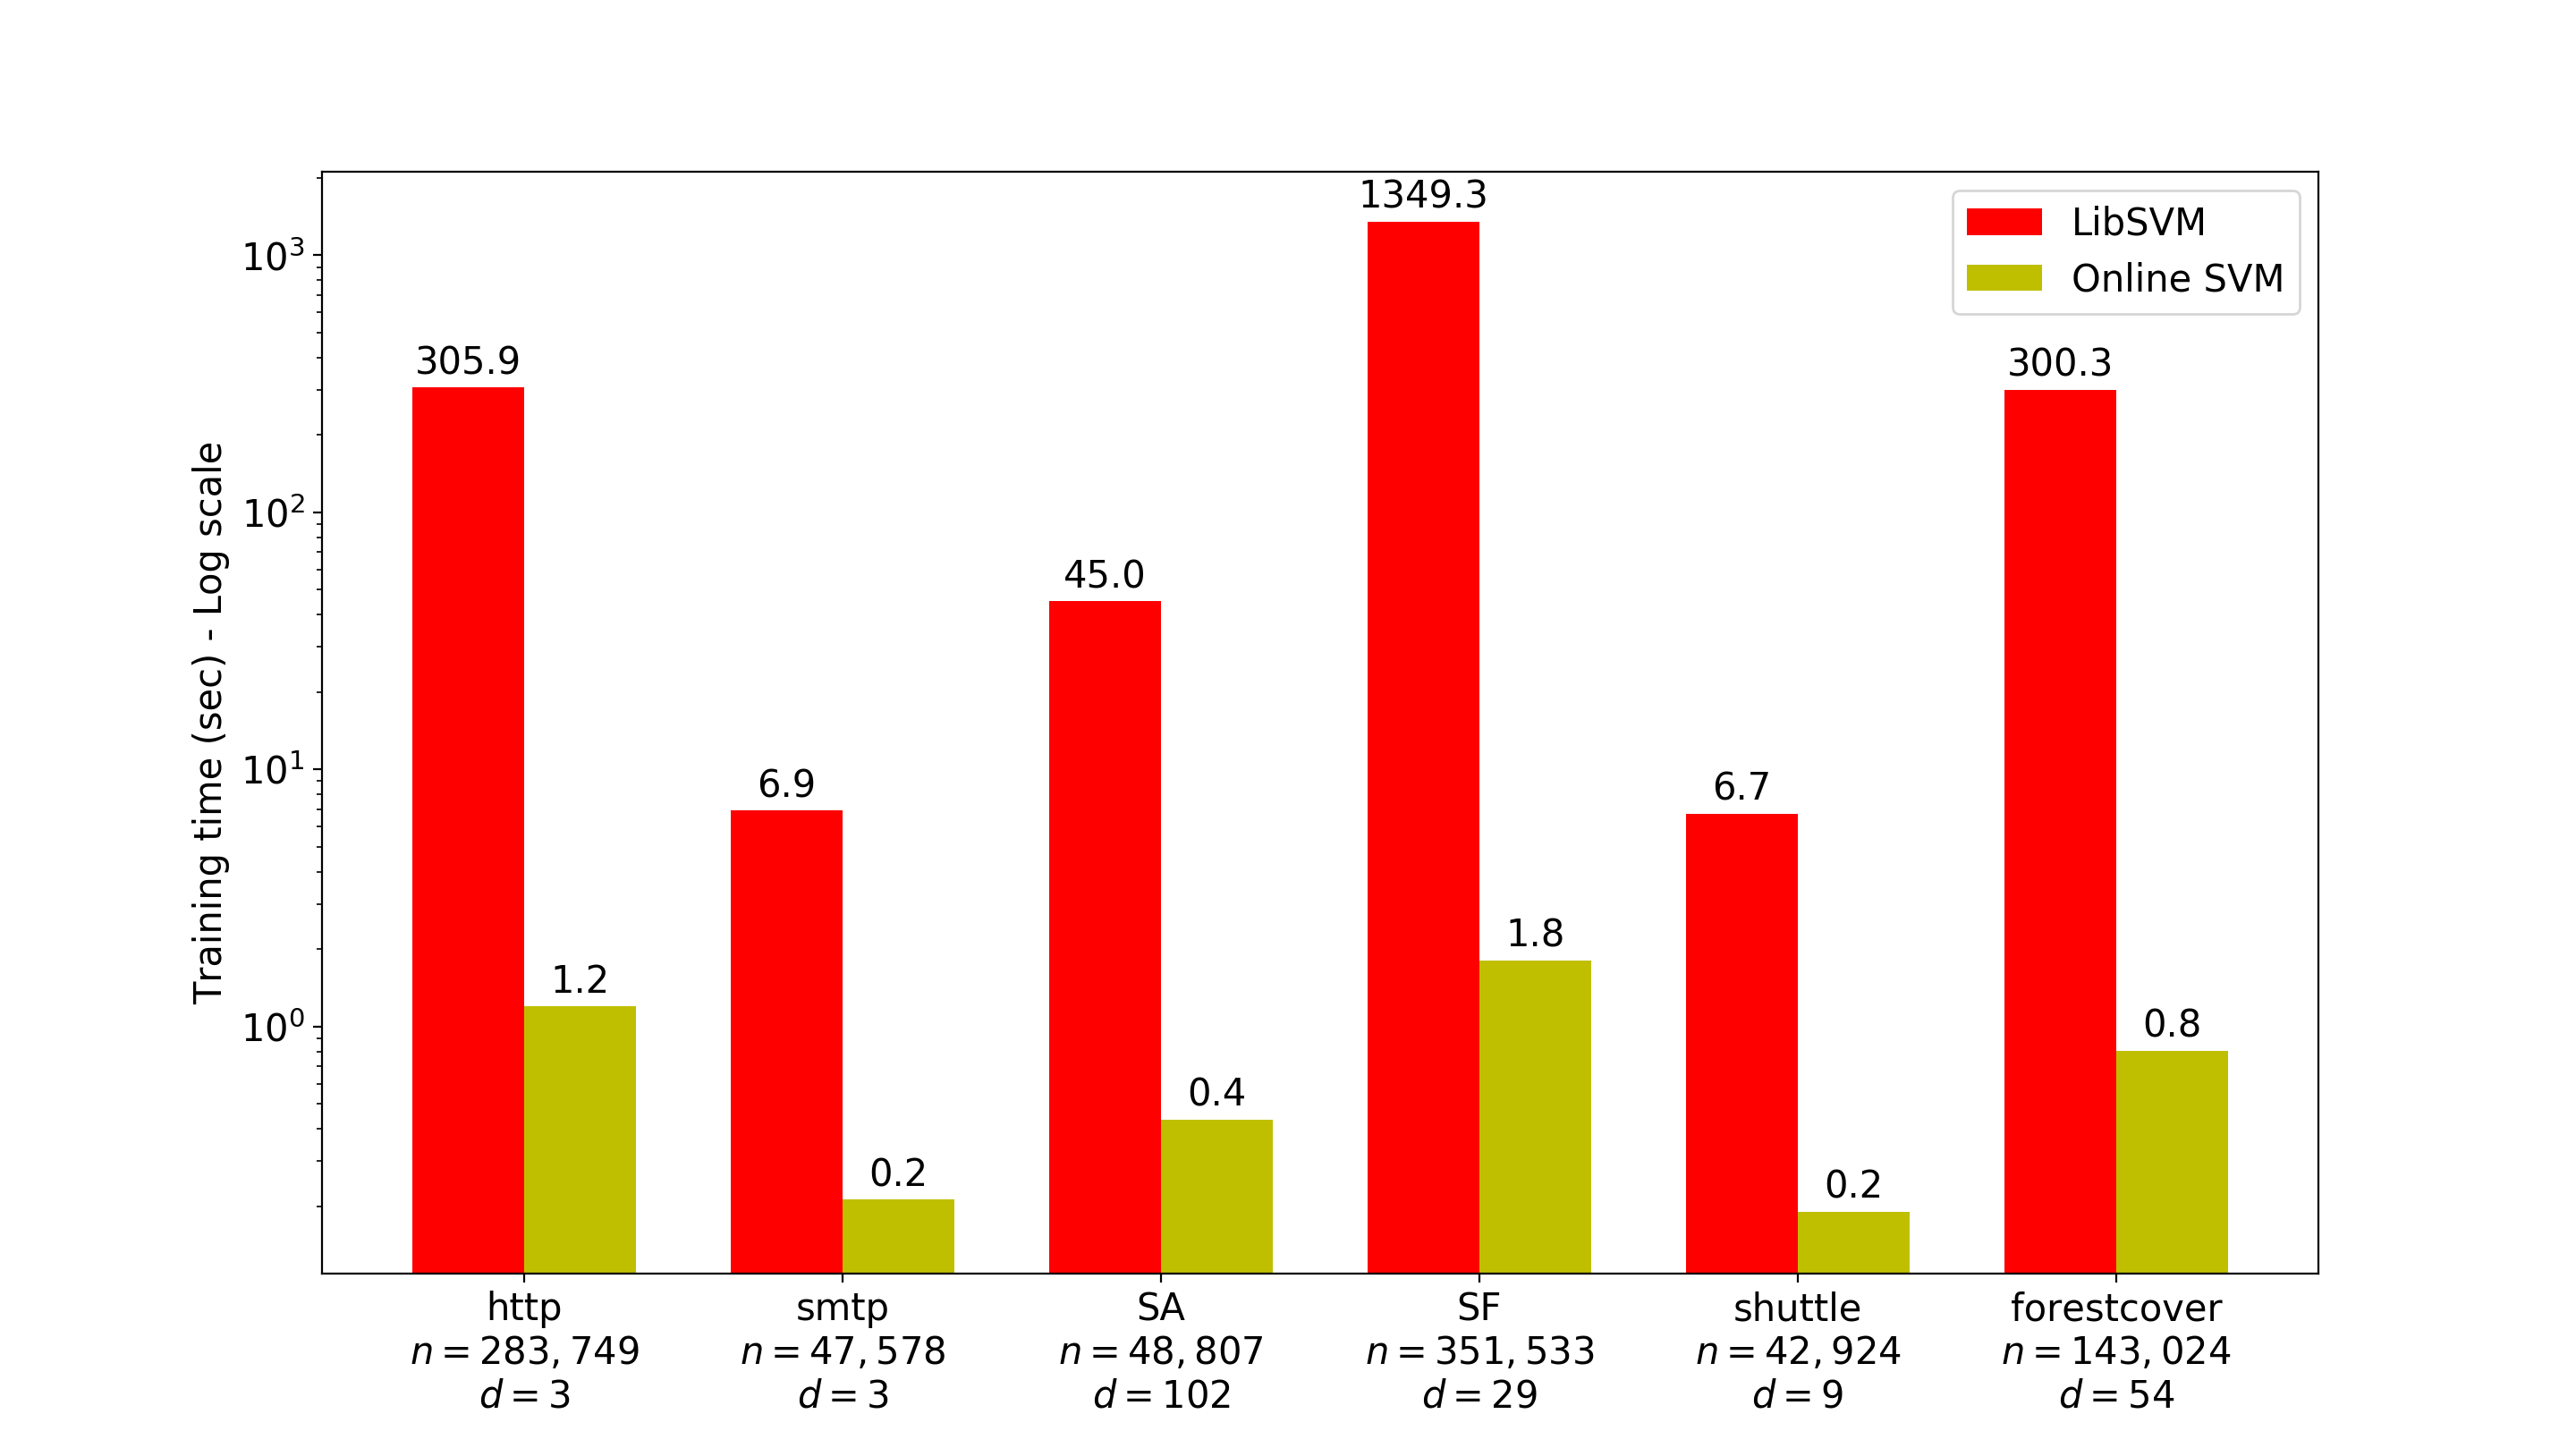
\includegraphics[width=11.5cm]{img/time_sgdocsvm.png}
\end{center}
}

\only<3>{
\begin{center}
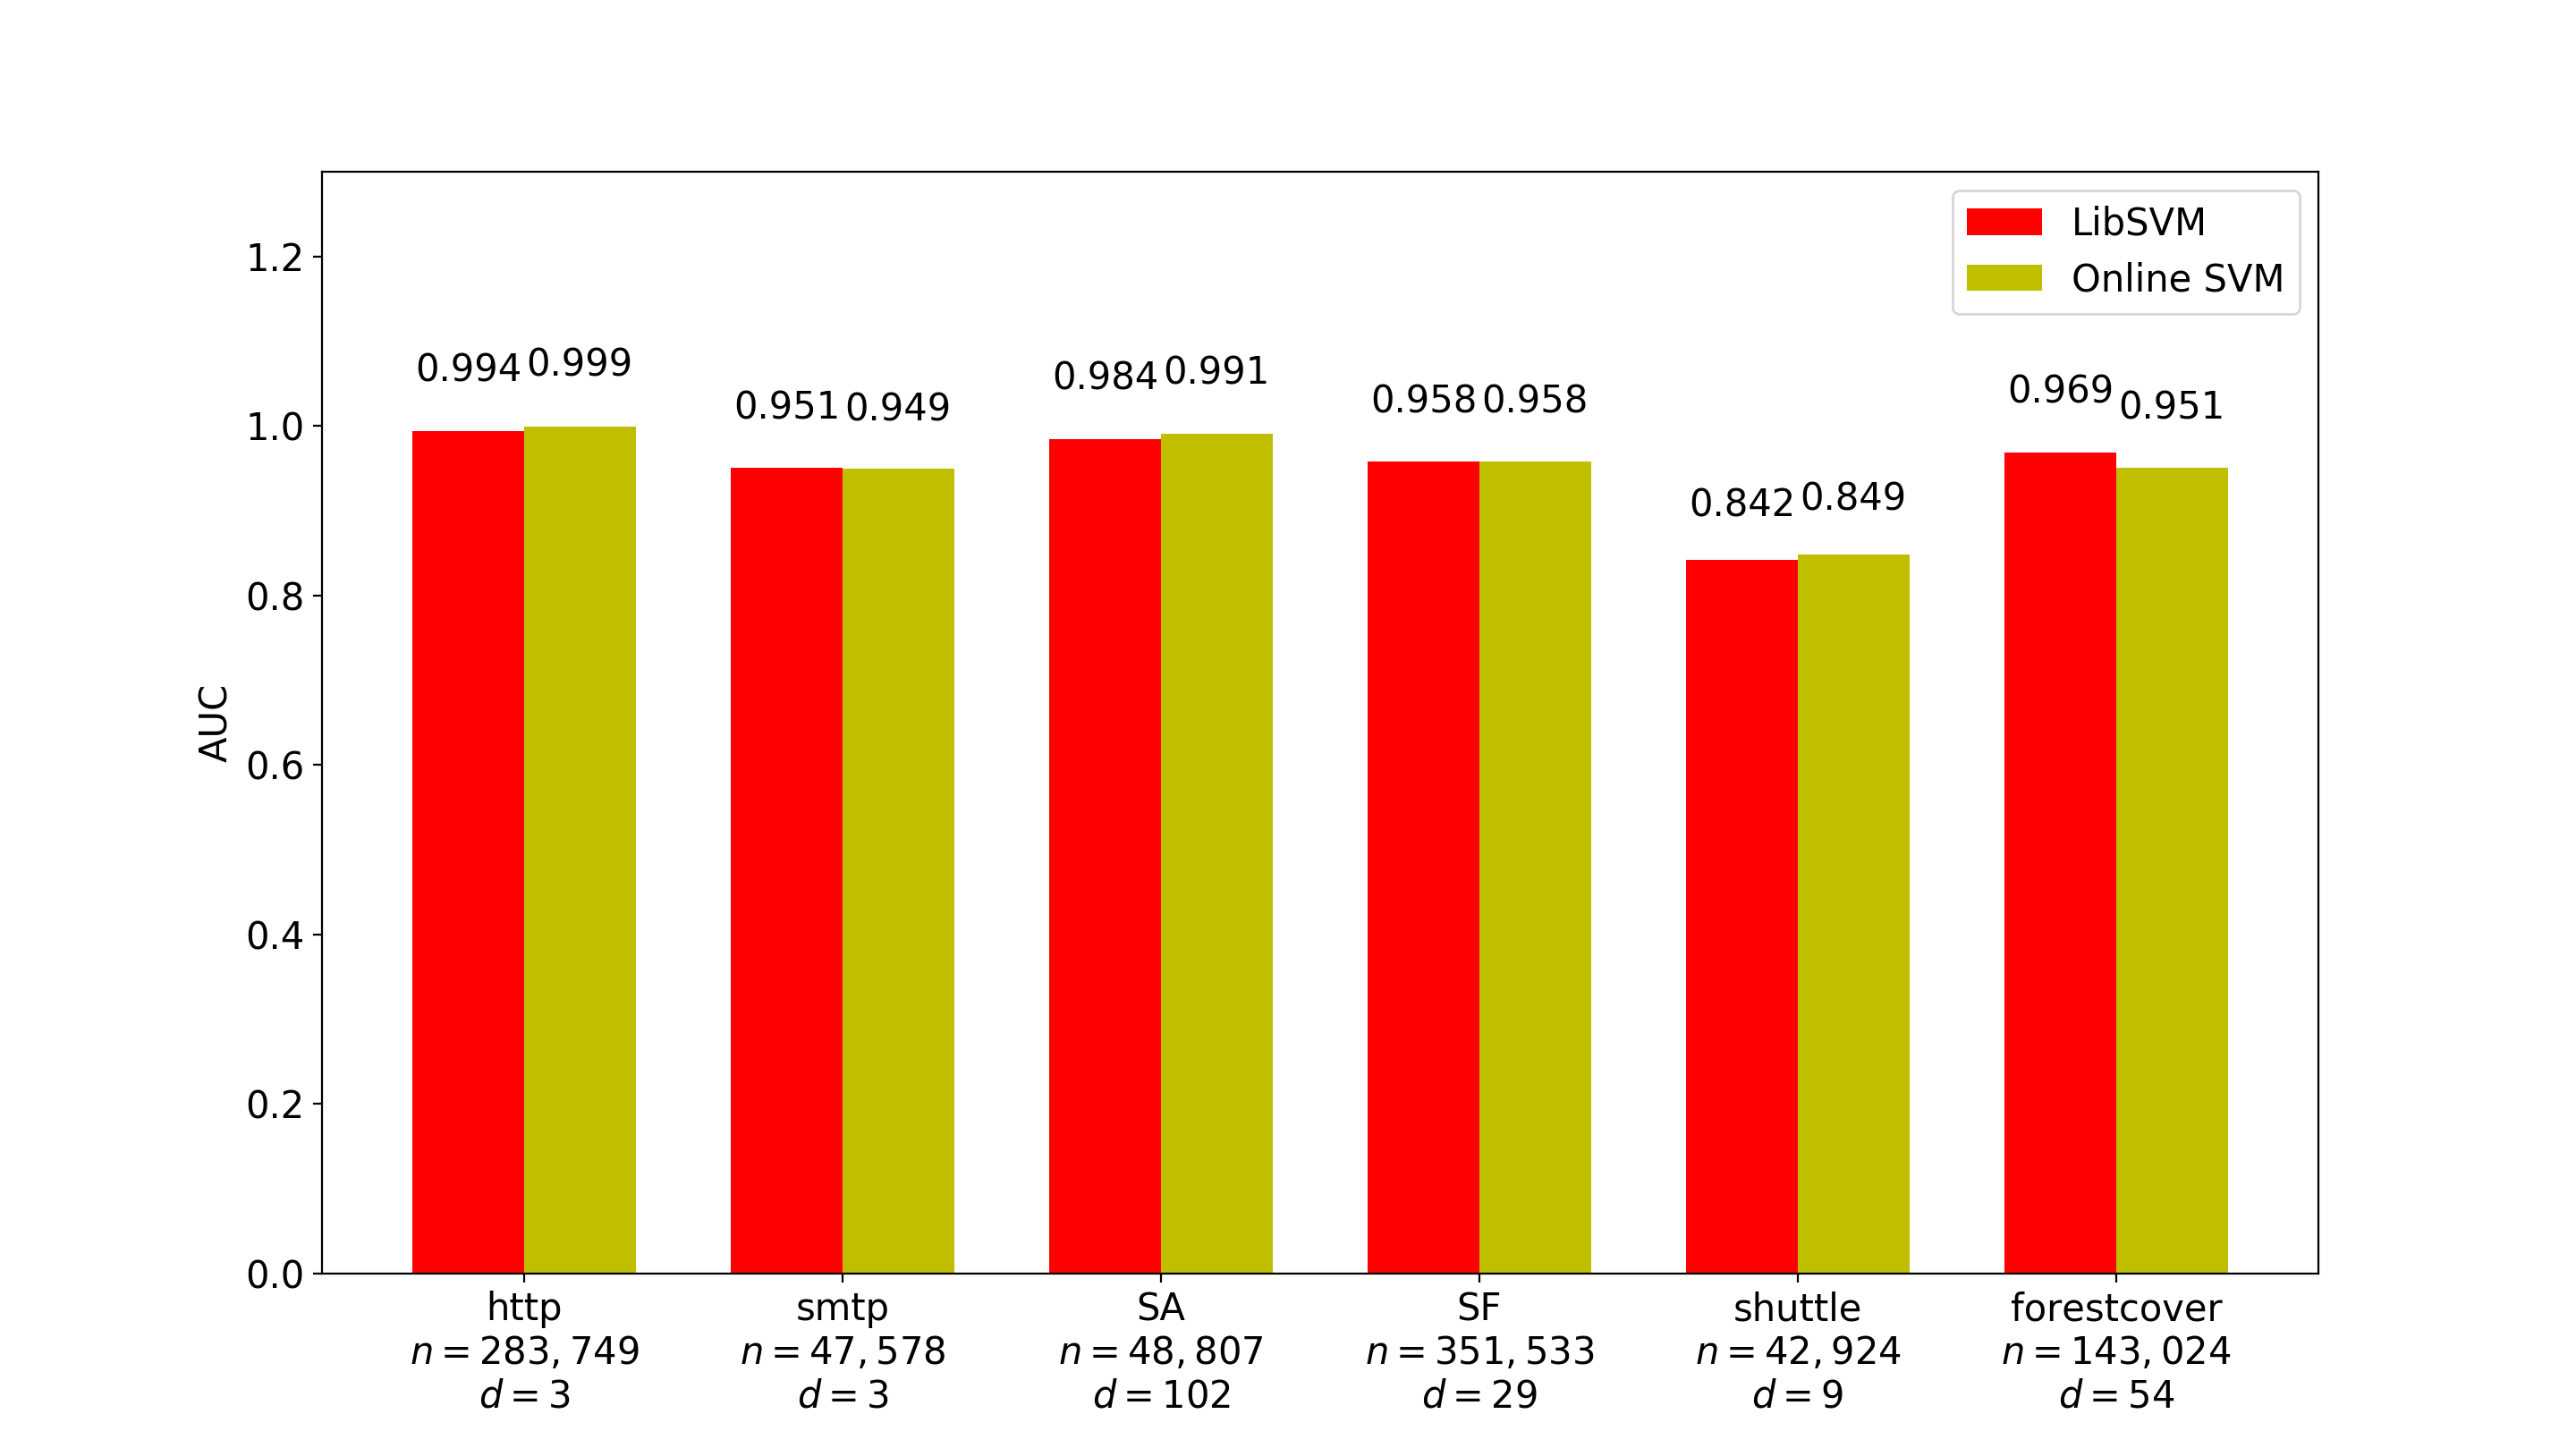
\includegraphics[width=11.5cm]{img/auc_sgdocsvm.png}
\end{center}
}

\end{frame}


\begin{frame}\frametitle{Future work}

Novelty detection for LOF: add \mintinline{python}{novelty} parameter in \mintinline{python}{__init__}
\begin{itemize}
  \item \mintinline{python}{novelty=False} (default): \mintinline{python}{predict}, \mintinline{python}{decision_function} and \mintinline{python}{scores_samples} raises \mintinline{python}{NotImplementedError}
  \item \mintinline{python}{novelty=True}: \mintinline{python}{fit_predict} raises \mintinline{python}{NotImplementedError}
\end{itemize}

\end{frame}


\begin{frame}\frametitle{Future work}

OutlierDetectionMixin
\begin{itemize}
  \item add \mintinline{python}{predict}? \mintinline{python}{decision_function}?
\end{itemize}

Anomaly detection benchmarks
\begin{itemize}
  \item one script per context (novelty vs outlier detection)
  \item convert fast benchmarks into examples
\end{itemize}

New estimators
\begin{itemize}
  \item SGDOneClassSVM
  \item Local Outlier Probabilities
  \item SVDD?
\end{itemize}

Documentation

\end{frame}


\begin{frame}\frametitle{Thanks to}
\begin{center}
@agramfort,  @jnothman, @ngoix, @amueller, @lesteve, @ogrisel, @TomDLT
\end{center}

\begin{center}
the scikit-learn community
\end{center}


\end{frame}



\end{document}



